\chapter{Schede di valutazione}

Nome e cognome: \_\_\_\_\_\_\_\_\_\_\_\_\_\_\_\_\_\_\_\_\_\_\_\_\_\_ \  Età:\_\_\_\_\_\_
\\\ \\\
\textbf{1$^{\circ}$visita:}  \ \ / \    /
\\\
\textbf{2$^{\circ}$visita:}  \ \ / \    /
\\\ \\\ \\\
\underline{\textbf{TEST LONTANO}}
\\\ \\\
\textbf{Distanza Interpupillare:}
\\\
OD: \_\_\_\_\_\_\_\_\_\_\_\_\_
\\\
OS: \_\_\_\_\_\_\_\_\_\_\_\_\_
\\\
OO: \_\_\_\_\_\_\_\_\_\_\_\_\_
\\\ \\\
\textbf{Refrazione:}
\\\
metodo: \_\_\_\_\_\_\_\_\_\_\_
\\\
Massimo positivo:
\\\
OD: sf \_\_\_\_\_\_\_\_ cil \_\_\_\_\_\_\_\_ asse \_\_\_\_\_\_\_\_ AV: \_\_\_\_\_\_\_\_ /10
\\\
OS: sf \_\_\_\_\_\_\_\_ cil \_\_\_\_\_\_\_\_ asse \_\_\_\_\_\_\_\_ AV: \_\_\_\_\_\_\_\_ /10
\\\
Minimo positivo:
\\\
OD: sf \_\_\_\_\_\_\_\_ cil \_\_\_\_\_\_\_\_ asse \_\_\_\_\_\_\_\_ AV: \_\_\_\_\_\_\_\_ /10
\\\
OS: sf \_\_\_\_\_\_\_\_ cil \_\_\_\_\_\_\_\_ asse \_\_\_\_\_\_\_\_ AV: \_\_\_\_\_\_\_\_ /10
\\\
Velocità:
\begin{table}[H]
\begin{tabular}{|c|c|c|} \hline
{\textbf{1}} & {\textbf{2}} & {\textbf{3}}\\ \hline
\end{tabular}
\end{table}
\\\ \\\
\textbf{Stereopsi Lontano:} \_\_\_\_\_\_\_\_
\\\ \\\
\textbf{Foria:} \_\_\_\_\_\_\_\_\_\_\_\_\_\_\_\_\_
\\\ \\\ \\\ \\\ \\\
\underline{\textbf{TEST VICINO}}
\\\ \\\
\textbf{PPC:}
\begin{table}[H]
\begin{tabular}{|c|c|c|c|} \hline
{\textbf{}} & {\textbf{Rott/Rec}} & {\textbf{Rott/Rec}}& {\textbf{Rott/Rec}}\\ \hline
\textbf{Pos. Diritto} & &  &  \\ \hline
\textbf{Pos. Alto} &  &  &  \\ \hline
\textbf{Pos. Basso} &  &  &  \\ \hline
\end{tabular}
\end{table}
\\\ \\\
fatica:
\begin{table}[H]
\begin{tabular}{|c|c|c|c|c|} \hline
{\textbf{1}} & {\textbf{2}} & {\textbf{3}} & {\textbf{4}} & {\textbf{5}}\\ \hline
\end{tabular}
\end{table}
\\\ \\\
soppressione: \_\_\_\_\_\_\_\_
\\\
deviazione: \_\_\_\_\_\_\_\_\_
\\\ \\\
\textbf{Forie:} 
\\\ 
metodo: \_\_\_\_\_\_\_\_\_\_\_
\begin{table}[H]
\begin{tabular}{|c|} \hline
{\textbf{Pos. Diritto \ \ \ \ \ \ \ \ \ \ \ \ \ \ \ \ \ \ \ \ \ \ \ } \\ \hline
\textbf{Pos. Alto \ \ \ \ \ \ \ \ \ \ \ \ \ \ \ \ \ \ \ \ \  \ \ \ \ \ } \\ \hline
\textbf{Pos. Basso \ \ \ \ \ \ \ \ \ \ \ \ \ \ \ \ \ \ \ \ \ \ \ \ } \\ \hline
\end{tabular}
\end{table}
\\\ \\\
fatica:
\begin{table}[H]
\begin{tabular}{|c|c|c|c|c|} \hline
{\textbf{1}} & {\textbf{2}} & {\textbf{3}} & {\textbf{4}} & {\textbf{5}}\\ \hline
\end{tabular}
\end{table}
\\\ \\\ \\\
\textbf{Cover test:}
\begin{table}[H]
\begin{tabular}{|c|c|c|c|c|c|c|c|c|c|} \hline
{\textbf{}} & {\ \ \textbf{1}\ \ } & {\ \ \textbf{2}\ \ } & {\ \ \textbf{3}\ \ } & {\ \ \textbf{4}\ \ } & {\ \ \textbf{5}\ \ } & {\ \ \textbf{6}\ \ } & {\ \ \textbf{7}\ \ } & {\ \ \textbf{8}\ \ } & {\ \ \textbf{9}\ \ \ }\\ \hline
\textbf{EXO}} &  &  &  &  &  &  &  &  & \\ \hline
\textbf{ESO}}  &  &  &  &  &  &  &  &  & \\ \hline
\end{tabular}
\end{table}

 \begin{figure}[h!]
	\centering
	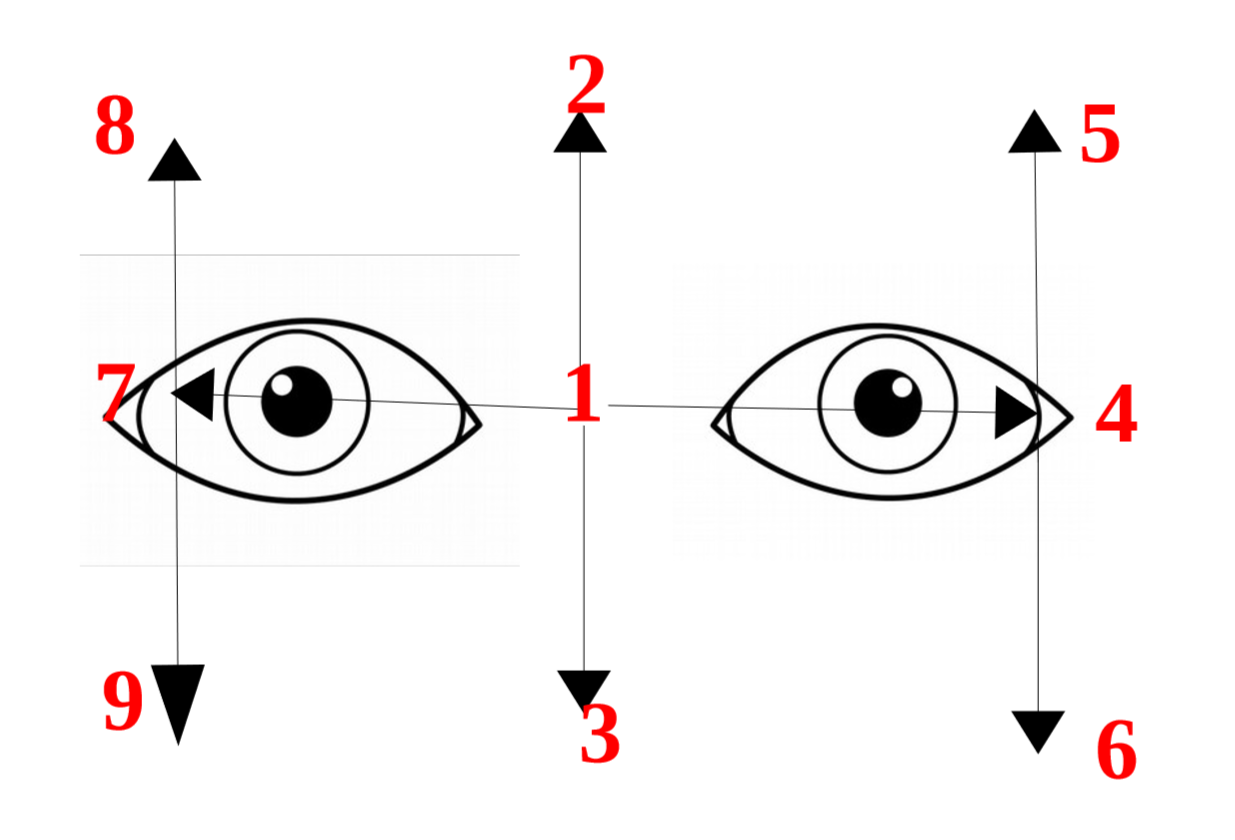
\includegraphics[scale=0.27]{source/immagini/posizioni_cover_test.png}
	\label{fig:issuexample}
\end{figure}
\\\ \\\
fatica:
\begin{table}[H]
\begin{tabular}{|c|c|c|c|c|} \hline
{\textbf{1}} & {\textbf{2}} & {\textbf{3}} & {\textbf{4}} & {\textbf{5}}\\ \hline
\end{tabular}
\end{table}
\\\ \\\
\textbf{AA}:
\\\
metodo: \_\_\_\_\_\_\_\_
\\\
\begin{table}[H]
\begin{tabular}{|c|c|c|c|} \hline
{\textbf{OD}} & {\ \ \ \ \ \ \ \ \ }  & {\ \ \ \ \ \ \ \ \ } & {\ \ \ \ \ \ \ \ \ } \\ \hline
\textbf{OS} & &  &  \\ \hline
\textbf{OO} &  &  &  \\ \hline
\end{tabular}
\end{table}
\\\ \\\
fatica:
\begin{table}[H]
\begin{tabular}{|c|c|c|c|c|} \hline
{\textbf{1}} & {\textbf{2}} & {\textbf{3}} & {\textbf{4}} & {\textbf{5}}\\ \hline
\end{tabular}
\end{table}
\\\ \\\
\textbf{Disparità di fissazione}: \_\_\_\_\_\_\_\_
\\\
\textbf{Stereopsi}: \_\_\_\_\_\_\_\_\_\_\_\_\_\_\_\_\_
\\\
\textbf{MEM}: 
\\\
OD: \_\_\_\_\_\_\_\_
\\\
OS: \_\_\_\_\_\_\_\_
